% -*- coding: utf-8 -*-
%-------------------------designed by zcf--------------
\documentclass[UTF8,a4paper,10pt]{ctexart}
\usepackage[left=3.17cm, right=3.17cm, top=2.74cm, bottom=2.74cm]{geometry}
\usepackage{amsmath}
\usepackage{graphicx,subfig}
\usepackage{float}
\usepackage{cite}
\usepackage{caption}
\usepackage{enumerate}
\usepackage{booktabs} %表格
\usepackage{multirow}
\usepackage{pythonhighlight}
\newcommand{\tabincell}[2]{\begin{tabular}{@{}#1@{}}#2\end{tabular}}  %表格强制换行
%-------------------------字体设置--------------
\usepackage{times} 
\newcommand{\yihao}{\fontsize{26pt}{36pt}\selectfont}           % 一号, 1.4 倍行距
\newcommand{\erhao}{\fontsize{22pt}{28pt}\selectfont}          % 二号, 1.25倍行距
\newcommand{\xiaoer}{\fontsize{18pt}{18pt}\selectfont}          % 小二, 单倍行距
\newcommand{\sanhao}{\fontsize{16pt}{24pt}\selectfont}  %三号字
\newcommand{\xiaosan}{\fontsize{15pt}{22pt}\selectfont}        % 小三, 1.5倍行距
\newcommand{\sihao}{\fontsize{14pt}{21pt}\selectfont}            % 四号, 1.5 倍行距
\newcommand{\banxiaosi}{\fontsize{13pt}{19.5pt}\selectfont}    % 半小四, 1.5倍行距
\newcommand{\xiaosi}{\fontsize{12pt}{18pt}\selectfont}            % 小四, 1.5倍行距
\newcommand{\dawuhao}{\fontsize{11pt}{11pt}\selectfont}       % 大五号, 单倍行距
\newcommand{\wuhao}{\fontsize{10.5pt}{15.75pt}\selectfont}    % 五号, 单倍行距
%-------------------------章节名----------------
\usepackage{ctexcap} 
\CTEXsetup[name={,、},number={ \chinese{section}}]{section}
\CTEXsetup[name={(,)},number={\chinese{subsection}}]{subsection}
\CTEXsetup[name={,.},number={\arabic{subsubsection}}]{subsubsection}
%-------------------------页眉页脚--------------
\usepackage{fancyhdr}
\pagestyle{fancy}
\lhead{\kaishu \leftmark}
% \chead{}
\rhead{\kaishu 机器学习实验报告}%加粗\bfseries 
\lfoot{}
\cfoot{\thepage}
\rfoot{}
\renewcommand{\headrulewidth}{0.1pt}  
\renewcommand{\footrulewidth}{0pt}%去掉横线
\newcommand{\HRule}{\rule{\linewidth}{0.5mm}}%标题横线
\newcommand{\HRulegrossa}{\rule{\linewidth}{1.2mm}}
%-----------------------伪代码------------------
\usepackage{algorithm}  
\usepackage{algorithmicx}  
\usepackage{algpseudocode}  
\floatname{algorithm}{Algorithm}  
\renewcommand{\algorithmicrequire}{\textbf{Input:}}  
\renewcommand{\algorithmicensure}{\textbf{Output:}} 
\usepackage{lipsum}  
\makeatletter
\newenvironment{breakablealgorithm}
  {% \begin{breakablealgorithm}
  \begin{center}
     \refstepcounter{algorithm}% New algorithm
     \hrule height.8pt depth0pt \kern2pt% \@fs@pre for \@fs@ruled
     \renewcommand{\caption}[2][\relax]{% Make a new \caption
      {\raggedright\textbf{\ALG@name~\thealgorithm} ##2\par}%
      \ifx\relax##1\relax % #1 is \relax
         \addcontentsline{loa}{algorithm}{\protect\numberline{\thealgorithm}##2}%
      \else % #1 is not \relax
         \addcontentsline{loa}{algorithm}{\protect\numberline{\thealgorithm}##1}%
      \fi
      \kern2pt\hrule\kern2pt
     }
  }{% \end{breakablealgorithm}
     \kern2pt\hrule\relax% \@fs@post for \@fs@ruled
  \end{center}
  }
\makeatother
%------------------------代码-------------------
\usepackage{xcolor} 
\usepackage{listings} 
\lstset{ 
breaklines,%自动换行
basicstyle=\small,
escapeinside=``,
keywordstyle=\color{ blue!70} \bfseries,
commentstyle=\color{red!50!green!50!blue!50},% 
stringstyle=\ttfamily,% 
extendedchars=false,% 
linewidth=\textwidth,% 
numbers=left,% 
numberstyle=\tiny \color{blue!50},% 
frame=trbl% 
rulesepcolor= \color{ red!20!green!20!blue!20} 
}
%------------超链接----------
\usepackage[colorlinks,linkcolor=black,anchorcolor=blue]{hyperref}
%------------------------TODO-------------------
\usepackage{enumitem,amssymb}
\newlist{todolist}{itemize}{2}
\setlist[todolist]{label=$\square$}
% for check symbol 
\usepackage{pifont}
\newcommand{\cmark}{\ding{51}}%
\newcommand{\xmark}{\ding{55}}%
\newcommand{\done}{\rlap{$\square$}{\raisebox{2pt}{\large\hspace{1pt}\cmark}}\hspace{-2.5pt}}
\newcommand{\wontfix}{\rlap{$\square$}{\large\hspace{1pt}\xmark}}
%------------------------水印-------------------
\usepackage{tikz}
\usepackage{xcolor}
\usepackage{eso-pic}

\newcommand{\watermark}[3]{\AddToShipoutPictureBG{
\parbox[b][\paperheight]{\paperwidth}{
\vfill%
\centering%
\tikz[remember picture, overlay]%
  \node [rotate = #1, scale = #2] at (current page.center)%
    {\textcolor{gray!80!cyan!30!magenta!30}{#3}};
\vfill}}}



%———————————————————————————————————————————正文———————————————————————————————————————————————
%----------------------------------------------
\begin{document}
\begin{titlepage}
    \begin{center}
    
\includegraphics[width=0.8\textwidth]{NKU.png}\\[1cm]    
    \textsc{\Huge \kaishu{\textbf{南\ \ \ \ \ \ 开\ \ \ \ \ \ 大\ \ \ \ \ \ 学}} }\\[0.9cm]
    \textsc{\huge \kaishu{\textbf{计\ \ 算\ \ 机\ \ 学\ \ 院}}}\\[0.5cm]
    \textsc{\Large \textbf{机器学习实验报告}}\\[0.8cm]
    \HRule \\[0.9cm]
    { \LARGE \bfseries 实验一\ 基于KNN的手写数字识别}\\[0.4cm]
    \HRule \\[2.0cm]
    \centering
    \textsc{\LARGE \kaishu{姓名\ :\ 王泳鑫}}\\[0.5cm]
    \textsc{\LARGE \kaishu{学号\ :\ 1911479}}\\[0.5cm]
    \textsc{\LARGE \kaishu{年级\ :\ 2019级}}\\[0.5cm]
    \textsc{\LARGE \kaishu{专业\ :\ 计算机科学与技术}}\\[0.5cm]
    \textsc{\LARGE \kaishu{指导教师\ :\ 卫金茂}}\\[0.5cm]
    \vfill
    {\Large \today}
    \end{center}
\end{titlepage}
%-------------摘------要--------------
\newpage
\thispagestyle{empty}
\renewcommand{\abstractname}{\kaishu \sihao \textbf{摘要}}
    \begin{abstract}

        \noindent  %顶格
        \textbf{\\\ 关键字:KNN ,Machine Learning , Deep Learning}\textbf{} \\\ \\\
    \end{abstract}
%----------------------------------------------------------------
\tableofcontents
%----------------------------------------------------------------
\newpage
\watermark{60}{10}{NKU}
\setcounter{page}{1}
%——————————————————————————————————————
\section{实验描述}
\subsection{实验内容}
给定semeion手写数字数据集,实现KNN分类算法
\subsection{实验要求}
基本要求:编程实现kNN算法;给定不同k值(1,3,5)情况下,kNN算法对手写数字的识别精度(要求采用留一法)
中级要求:将实验过程结果等图示展出

%——————————————————————————————————————
\section{代码实现}
\subsection{kNN分类算法}

该函数的功能就是使用k-邻近算法将每组数据划分到某个类中,其算法伪代码如下:

\begin{enumerate}
   \item 计算已知类别数据集中的点和当前点的距离;
   \item 按照距离递增次序排序;
   \item 选取与当前点距离最小的k个点;
   \item 确定前k个点所在类别的出现频率;
   \item 返回前k个点出现频率最高的类别作为当前点的预测分类。
\end{enumerate}
\begin{python}
   def classify0(inX,dataSet,labels,k):#knn分类器
   #首先计算已知类别数据集与当前点的距离
   dataSetSize=dataSet.shape[0]#读取数据集的行数,声明为dataSetSize
   diffMat = tile(inX,(dataSetSize,1))-dataSet#
   sqDiffMat = diffMat**2#平方
   sqDistances = sqDiffMat.sum(axis=1)#相加
   distances = sqDistances**0.5#开方


   #按照距离递增次序排序
   sortedDistindicies = distances.argsort()#返回排序结果的索引
   classCount = {}#新建一个词典用来计数

   #选取与当前点距离最小的k个点并且确定出现频率
   for i in range(k):
       voteIlabel = labels[sortedDistindicies[i]]
       classCount[voteIlabel] = classCount.get(voteIlabel,0)+1

   #将出现频率进行排序
   sortedClassCount = sorted(classCount.items(),key=operator.itemgetter(1),reverse=True)
   return sortedClassCount[0][0]

\end{python}

\subsection{数据集处理}

本次实验采用semeion数据集,该数据集每一条数据项,都是由256个0或1组成(相当于16*16的阴影),同时后面紧跟着一个大小为10的独热码来标注它的分类,
因此对于该数据集,我们需要将前面256大小的数据作为计算距离的dataset,后面的独热码作为可以判断分类的label。

\begin{python}
   def datareading(filename):
    #读取文件
    fo=open(filename)
    data = fo.readlines()
    fo.close()

    row = len(data)#计算数据项的数量
    dataMat = zeros((row,256))#初始化为零矩阵
    dataLabels = []#新建一个列表,用来存储label

    for i in range(row):
        vals = data[i].split()
        dataMat[i,:] = vals[0:256]
        dataLabels.append(vals[256:].index('1'))

    return dataMat,dataLabels
\end{python}

\subsection{测试与验证}
实验要求使用留一法来进行验证,留一法就是每次只留下一个样本做测试集,其它样本做训练集,
如果有n个样本,则需要训练n次,测试n次。
\begin{python}
   def test():
    dataMat,dataLabels = datareading('D:\\Data\\semeion.data')
    m = dataMat.shape[0]
    testnum = int(m*0.1)
    TNum = 0
    k=3
    for i in range(testnum):
        ans = classify0(dataMat[i,:],dataMat[testnum:,:],dataLabels[testnum:],k)
        if(ans==dataLabels[i]): TNum+=1
    print("When k is ",k,",the Precision is",TNum/testnum)
\end{python}

%——————————————————————————————————————
\section{实验结果展示与分析}
对于指定k进行测试,当k为(1,3,5)时,测试结果如图\ref{fig:1}所示
\begin{figure}[H]
    \centering
    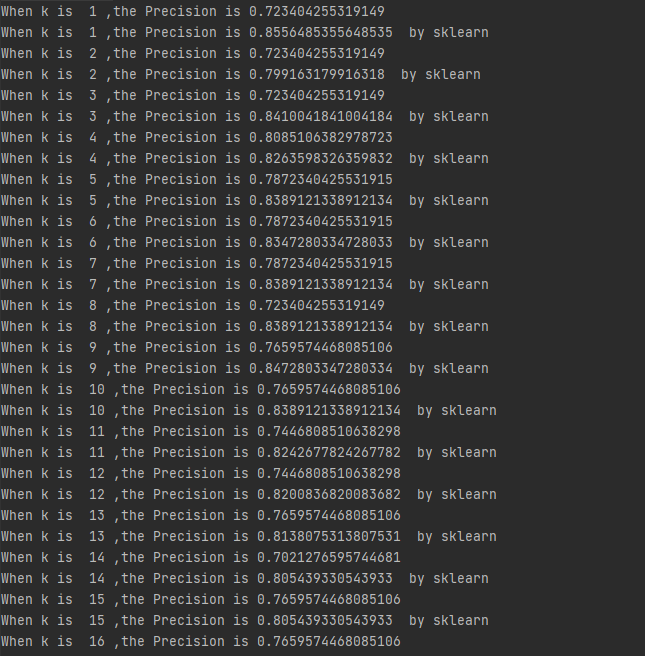
\includegraphics[scale=0.7]{2.png}
    \caption{kNN测试结果}
    \label{fig:1}
\end{figure}
这幅图中也包含了利用sklearn中knn分类算法得到预测结果,我所写的程序在不同k值的情况下得到的结果如下图\ref{fig:1}所示:
\begin{figure}[H]
    \centering
    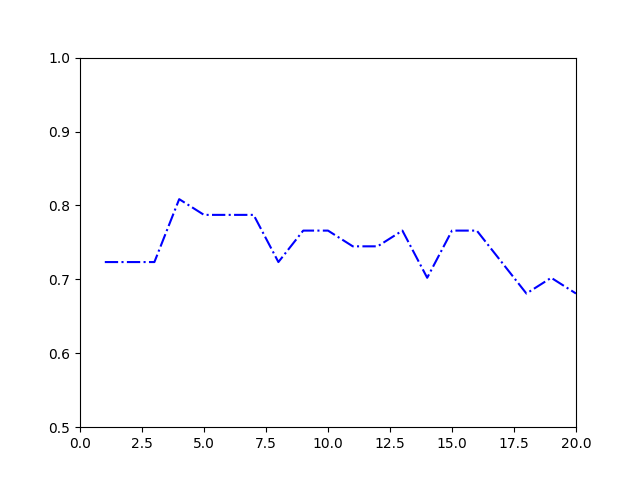
\includegraphics[scale=0.7]{3.png}
    \caption{myplot}
    \label{fig:1}
\end{figure}


%----------------------------------------------------------------

%----------------------------------------------------------------
\bibliographystyle{plain}
\end{document}
